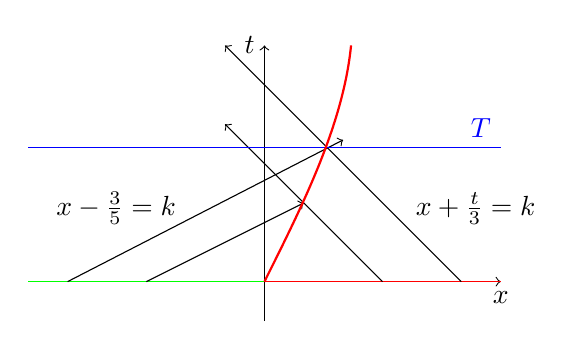
\begin{tikzpicture}

\draw[->] (-3, 0) -- (3,0) node[below] {$x$};
\draw[->] (0, -0.5) -- (0,3) node[left] {$t$};

\draw[green] (-3,0) -- (0,0);
\draw[red] (0,0) -- (3,0);

\draw[->] (-1.5,0) -- (0.5,1);
\draw[->] (1.5,0) -- (-0.5,2);
\draw[->] (-2.5,0) -- (1,1.8);
\draw[->] (2.5,0) -- (-0.5,3);

\draw[blue] (-3,1.7) -- (3,1.7) node[above left] {$T$};


\draw[thick, red] (0,0) .. controls (0.5,1) and (1,2) .. (1.1,3);


\draw (-1,0.6) node[above left] {$x-\frac{3}{5} = k$};
\draw (1.8,0.6) node[above right] {$x+\frac{t}{3} = k$};


\end{tikzpicture}